% Created 2019-08-12 lun. 16:02
% Intended LaTeX compiler: pdflatex
\documentclass[9pt, technote, a4paper]{ieeeconf}
\usepackage[utf8]{inputenc}
\usepackage[T1]{fontenc}
\usepackage{graphicx}
\usepackage{grffile}
\usepackage{longtable}
\usepackage{wrapfig}
\usepackage{rotating}
\usepackage[normalem]{ulem}
\usepackage{amsmath}
\usepackage{textcomp}
\usepackage{amssymb}
\usepackage{capt-of}
\usepackage{hyperref}
\usepackage[most]{tcolorbox}
\usepackage{siunitx}
\usepackage{amsmath,amssymb,amsfonts, cases}
\usepackage{algorithmic, graphicx, textcomp}
\usepackage{xcolor, import, hyperref}
\usepackage[USenglish, english]{babel}
\setcounter{footnote}{1}
%%% Local Variables:
%%% TeX-master: "poster"
%%% End:

% ==============================================================================
% Packages
% ==============================================================================
\usepackage[utf8]{inputenc}
\usepackage[T1]{fontenc}
\usepackage[        % use biblatex for bibliography
    backend=biber,  % use biber backend (bibtex replacement) or bibtex
    style=ieee,     % bib style
    natbib=true,    % allow natbib commands
    hyperref=true,  % activate hyperref support
    backref=false,  % activate backrefs
    isbn=false,     % don't show isbn tags
    url=false,      % don't show url tags
    doi=false,      % don't show doi tags
    urldate=long,   % display type for dates
    maxnames=3,     %
    minnames=1,     %
    maxbibnames=5,  %
    minbibnames=3,  %
    maxcitenames=2, %
    mincitenames=1  %
]{biblatex}

\usepackage[english]{babel}  % Last language is main language
\usepackage{lmodern}         % Latin Modern Font
\usepackage{amssymb}
\usepackage{gensymb}         % Generic symbols for both text and math mode
\usepackage{amsmath}         % Main math Package
\usepackage{mathtools}       % Extension package to amsmath
\usepackage{amsthm}          % Typesetting theorems (AMS style)
\usepackage{amsfonts}        % More fonts from the AMS
\usepackage{textcomp}        % provide many text symbols
\usepackage{xstring}         % Utils to manipulate strings
\usepackage{etoolbox}        % Add basic if/then and usefull functions
\usepackage{esvect}          % Beautyfull vectors
\usepackage{graphicx}        % Enhanced support for graphics
\usepackage{grffile}         % Used by matlab2tikz
\usepackage{microtype}       % typographic tuning
\usepackage{setspace}        % for line spacing, e.g. \onehalfspacing
\usepackage{csquotes}        % Nice display of quotations
\usepackage{blindtext}       % package for blind text
\usepackage{steinmetz}       % For phase symbol
\usepackage[load-configurations=abbreviations]{siunitx} % SI units
\usepackage{caption}
\usepackage{subcaption}
\usepackage{wrapfig}         % Wrap text around figure
\usepackage{tikz}
\usepackage{array}     % Basic table support
\usepackage{tabularx}  % Great for auto-sizing columns
\usepackage{booktabs}  % Professional-looking layout
\usepackage[most]{tcolorbox}
\usepackage[framemethod=TikZ]{mdframed}
\usepackage{enumitem}
\usepackage[table]{xcolor}%
\usepackage{authblk}

\usepackage[cache=false]{minted}
% ==============================================================================

\renewcommand\Affilfont{\itshape\large}

% ==============================================================================
% Remove credentials of tikzposter
\tikzposterlatexaffectionproofoff
% ==============================================================================


% ==============================================================================
% Change MakeTitle command
% ==============================================================================
\makeatletter
\newcommand\insertlogoright[2][]{\def\@insertlogoright{\includegraphics[#1]{#2}}}
\newcommand\insertlogoleft[2][]{\def\@insertlogoleft{\includegraphics[#1]{#2}}}
\newlength\LogoSep
\setlength\LogoSep{60pt}

\insertlogoright[height=6cm]{./img/logo_esrf.pdf}
\insertlogoleft[height=6cm]{./img/logo_pml.pdf}

\renewcommand\maketitle[1][]{  % #1 keys
    \normalsize
    \setkeys{title}{#1}
    % Title dummy to get title height
    \node[transparent,inner sep=\TP@titleinnersep, line width=\TP@titlelinewidth, anchor=north, minimum width=\TP@visibletextwidth-2\TP@titleinnersep]
        (TP@title) at ($(0, 0.5\textheight-\TP@titletotopverticalspace)$) {\parbox{\TP@titlewidth-2\TP@titleinnersep}{\TP@maketitle}};
    \draw let \p1 = ($(TP@title.north)-(TP@title.south)$) in node {
        \setlength{\TP@titleheight}{\y1}
        \setlength{\titleheight}{\y1}
        \global\TP@titleheight=\TP@titleheight
        \global\titleheight=\titleheight
    };

    % Compute title position
    \setlength{\titleposleft}{-0.5\titlewidth}
    \setlength{\titleposright}{\titleposleft+\titlewidth}
    \setlength{\titlepostop}{0.5\textheight-\TP@titletotopverticalspace}
    \setlength{\titleposbottom}{\titlepostop-\titleheight}

    % Title style (background)
    % \TP@titlestyle

    % Title node
    \node[inner sep=\TP@titleinnersep, line width=\TP@titlelinewidth, anchor=north, minimum width=\TP@visibletextwidth-2\TP@titleinnersep]
        at (0,0.5\textheight-\TP@titletotopverticalspace)
        (title)
        {\parbox{\TP@titlewidth-2\TP@titleinnersep}{\TP@maketitle}};

    \node[inner sep=0pt,anchor=west]
      at ([xshift=\LogoSep]title.west)
      {\@insertlogoleft};

    \node[inner sep=0pt,anchor=east]
      at ([xshift=-\LogoSep]title.east)
      {\@insertlogoright};

    % Settings for blocks
    \normalsize
    \setlength{\TP@blocktop}{\titleposbottom-\TP@titletoblockverticalspace}
}

\def\title#1{\gdef\@title{\scalebox{\TP@titletextscale}{%
      \begin{minipage}[t]{\linewidth}
        \centering
        #1
        \par
        \vspace{0.5em}
      \end{minipage}%
    }}}
\makeatother
% ==============================================================================


% ==============================================================================
% Create Table Environment
% ==============================================================================
\makeatletter
\newcounter{tablecounter}
\newenvironment{tikztable}[1][]{
  \def \rememberparameter{#1}
  \vspace{10pt}
  \refstepcounter{tablecounter}
  \begin{center}
  }{
    \ifx\rememberparameter\@empty
    \else
    \\[10pt]
    {\small Tab.~\thetablecounter: \rememberparameter}
    \fi
  \end{center}
}
\makeatother
% ==============================================================================


% ==============================================================================
% Change block style
% ==============================================================================
\defineblockstyle{customstyle}{
    titlewidthscale=1, bodywidthscale=1, titlecenter,
    titleoffsetx=0pt, titleoffsety=0pt, bodyoffsetx=0pt, bodyoffsety=0pt,
    bodyverticalshift=0pt, roundedcorners=2, linewidth=2mm,
    titleinnersep=5mm, bodyinnersep=1cm
}{
    \begin{scope}[line width=\blocklinewidth, rounded corners=\blockroundedcorners]
        \ifBlockHasTitle %
           \draw[color=blocktitlebgcolor, fill=blocktitlebgcolor] (blockbody.south west) rectangle (blocktitle.north east);
           \draw[color=blocktitlebgcolor, fill=blockbodybgcolor] (blockbody.south west) rectangle (blockbody.north east);
        \else
           \draw[color=blocktitlebgcolor, fill=blockbodybgcolor] (blockbody.south west) rectangle (blockbody.north east);
        \fi
    \end{scope}
}
\usetheme{Default}
\usebackgroundstyle{Empty}
% ==============================================================================


% ==============================================================================
% Simple TCMBOX environment
% ==============================================================================
\definecolor{maincolor}{HTML}{0066A7}

\newtcbox{\tcmbox}[1][blue]{colback=maincolor!5!white, colframe=maincolor,
  nobeforeafter,math upper,tcbox raise base, boxrule=1mm, boxsep=4mm}
\newtcolorbox{cbox}[3][]{colback=maincolor!5!white, colframe=maincolor, fonttitle=\bfseries, size=normal, toptitle=3mm, botttomtitle=3mm, boxrule=1mm, title=#1, #3}
% ==============================================================================


% ==============================================================================
\newlength{\seplinewidth}
\newlength{\seplinesep}
\setlength{\seplinewidth}{1mm}
\setlength{\seplinesep}{2mm}

\newcommand*{\sepline}{%
  \par
  \vspace{\dimexpr\seplinesep+.5\parskip}%
  \cleaders\vbox{%
    \begingroup % because of color
    \color{maincolor}%
    \hrule width\linewidth height\seplinewidth
    \endgroup
  }\vskip\seplinewidth
  \vspace{\dimexpr\seplinesep-.5\parskip}%
}
% ==============================================================================

% ==============================================================================
\definecolor{mycolor1}{RGB}{79,115,193}
\definecolor{mycolor2}{RGB}{213,91,53}
% ==============================================================================

% ==============================================================================
\AtBeginBibliography{\small}
% ==============================================================================
\author{\IEEEauthorblockN{Dehaeze Thomas\IEEEauthorrefmark{*} and Collette Christophe} \\ \IEEEauthorblockA{Precision Mechatronics Laboratory, ULB\\ Brussels, Belgium\\ Email: \IEEEauthorrefmark{*}dehaeze.thomas@gmail.com}}
\date{2019-08-12}
\title{On the Design of Complementary Filters for Control}
\hypersetup{
 pdfauthor={\IEEEauthorblockN{Dehaeze Thomas\IEEEauthorrefmark{*} and Collette Christophe} \\ \IEEEauthorblockA{Precision Mechatronics Laboratory, ULB\\ Brussels, Belgium\\ Email: \IEEEauthorrefmark{*}dehaeze.thomas@gmail.com}},
 pdftitle={On the Design of Complementary Filters for Control},
 pdfkeywords={},
 pdfsubject={},
 pdfcreator={Emacs 26.2 (Org mode 9.2.5)},
 pdflang={English}}
\begin{document}

\maketitle
\bibliographystyle{IEEEtran}

\begin{abstract}
Abstract text to be done
\end{abstract}

\begin{IEEEkeywords}
complementary filters, h-infinity, feedback control
\end{IEEEkeywords}

\section{Introduction}
\label{sec:orgb15ebed}
  \label{sec:introduction}
The basic idea of a complementary filter involves taking two or more sensors, filtering out unreliable frequencies for each sensor and combining the filtered outputs to get a better estimate throughout the entire bandwidth of the system.
To achieve this, the sensors included in the filter should complement one another by performing better over specific parts of the system bandwidth.
A set of filters is said to be complementary if the sum of their transfer functions is equal to one at all frequencies, (i.e.) its magnitude is one and its phase is zero.

The proper design of this particular kind of filter is of primary importance in a wide range of applications.
Often, multiple sensors with different noise or dynamical properties are used to measure the same physical quantity.
In such case, complementary filters can be used to merge the sensors and forms a "super sensor" that has gives a better estimate of the physical quantity over a wider bandwidth.
This is called sensor blending or sensor fusion.

This is widely used for the attitude estimation of unmanned aerial vehicles using various kind of sensors (accelerometers, gyroscopes, vision sensors, inclinometer) \cite{zimmermann92_high_bandw_orien_measur_contr,corke04_inert_visual_sensin_system_small_auton_helic,min15_compl_filter_desig_angle_estim}.

\cite{shaw90_bandw_enhan_posit_measur_using_measur_accel} Fast position measurement of flexible structure

\cite{matichard15_seism_isolat_advan_ligo} (relative displacement measurement at low frequencies with inertial at high frequencies)

\cite{hua04_polyp_fir_compl_filter_contr_system}

\cite{collette15_sensor_fusion_method_high_perfor}
The design methods for such filters goes from simple analytical formulas

\cite{corke04_inert_visual_sensin_system_small_auton_helic}

\cite{min15_compl_filter_desig_angle_estim}
\cite{jensen13_basic_uas}

\cite{shaw90_bandw_enhan_posit_measur_using_measur_accel}
\cite{zimmermann92_high_bandw_orien_measur_contr}
\cite{matichard15_seism_isolat_advan_ligo}
\cite{collette15_sensor_fusion_method_high_perfor}

\cite{hua05_low_ligo}
\cite{hua04_polyp_fir_compl_filter_contr_system}
\cite{matichard15_seism_isolat_advan_ligo}

\cite{mahony08_nonlin_compl_filter_special_orthog_group}

\cite{pascoal99_navig_system_desig_using_time}

\cite{jensen13_basic_uas} (feedback system, P, PI, classical control theory for filter design)
\cite{brown72_integ_navig_system_kalman_filter}

\cite{pascoal99_navig_system_desig_using_time}

\cite{min15_compl_filter_desig_angle_estim}
Although
In this paper, we propose
The body of the paper consists of five parts followed by a conclusion.

\section{H-Infinity synthesis of complementary filters}
\label{sec:org303afb5}
  \label{sec:hinf_filters}
First order complementary filters are easy to synthesize. For instance, one can use the following filters
\begin{equation}
H_H(s) = \frac{s/\w_0}{1 + s/\w_0}; \quad H_L(s) = \frac{1}{1 + s/\w_0}
\end{equation}
with \(\w_0\) is the tuning parameter corresponding to the crossover frequency of the filters.

However, the manual design of higher order complementary filters is far more complex and we have to use an automatic synthesis technique.


As shown in Sec. \ref{sec:trans_perf}, most of the performance requirements can be expressed as upper bounds on the magnitude of the complementary filters.

Thus, the \(\mathcal{H}_\infty\) framework seems adapted and we here propose a technique to synthesis complementary filters while specifying uppers bounds on their magnitudes.

\subsection{\(\hinf\) problem formulation}
\label{sec:org9dcb2b1}
   \label{sec:hinf_conf}
In this section, we formulate the \(\hinf\) problem for the synthesis of complementary filters.

The synthesis objective is to shape an high pass filter \(H_H\) and a low pass filter \(H_L\) while ensuring their complementary property (\(H_H + H_L = 1\)).

To do so, we define two weighting functions \(w_L\) and \(w_H\) that will respectively used to shape \(H_L\) and \(H_H\).

The synthesis problem is then
\begin{subnumcases}{\text{Find } H_L, H_H \text{ such that}}
  H_L \text{ and } H_H \text{ are stable} \label{eq:hinf_cond_stability}\\
  H_L + H_H = 1 \label{eq:hinf_cond_complementarity} \\
  |w_L H_L| \le 1 \quad \forall\omega \label{eq:hinf_cond_hl} \\
  |w_H H_H| \le 1 \quad \forall\omega \label{eq:hinf_cond_hh}
\end{subnumcases}


To express this synthesis problem into an \(\hinf\) synthesis problem, we define the following generalized plant \(P\) (also shown on Fig. \ref{fig:sf_hinf_filters_plant_b}):
\begin{equation}
\label{eq:generalized_plant}
  \colvec{w\\u} = P \colvec{z_H \\ z_L \\ v}; \quad P = \begin{bmatrix} w_H & -w_H \\ 0 & w_L \\ 1 & 0 \end{bmatrix}
\end{equation}

\begin{figure}[htbp]
\centering
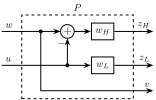
\includegraphics[scale=1]{./figs/sf_hinf_filters_plant_b.pdf}
\caption{\label{fig:sf_hinf_filters_plant_b}
Generalized plant for the synthesis of the complementary filters}
\end{figure}

The \(\hinf\) synthesis objective is then to design a stable filter \(H_L\) (Fig. \ref{fig:sf_hinf_filters_b}) such that the \(\mathcal{H}_\infty\) norm of the transfer function from \(w\) to \([z_H, \ z_L]\) is less than \(1\):
\begin{equation}
  \hnorm{\begin{matrix} (1 - H_L) w_H \\ H_L w_L \end{matrix}} \le 1
\end{equation}
Which is equivalent to
\begin{equation}
\label{eq:hinf_problem}
  \hnorm{\begin{matrix} H_H w_H \\ H_L w_L \end{matrix}} < 1 \text{ by choosing } H_H = 1 - H_L
\end{equation}

\begin{figure}[htbp]
\centering
\includegraphics[scale=1]{./figs/sf_hinf_filters_b.pdf}
\caption{\label{fig:sf_hinf_filters_b}
\(\hinf\text{-synthesis}\) of complementary filters}
\end{figure}

Performance conditions \eqref{eq:hinf_cond_hl} and \eqref{eq:hinf_cond_hl} are satisfied by \eqref{eq:hinf_problem}.
Complementary condition \eqref{eq:hinf_cond_complementarity} is satisfied by design: \(H_H = 1 - H_L\) and thus \(H_L + H_H = 1\).
The stability condition \eqref{eq:hinf_cond_stability} is guaranteed by the \(H_\infty\) synthesis (\textbf{reference}).


Using this synthesis method, we are then able to shape at the same time the high pass and low pass filters while ensuring their complementary.

\subsection{Control requirements as \(\mathcal{H}_\infty\) norm of complementary filters}
\label{sec:orgb7d25ea}
As presented in Sec. \ref{sec:trans_perf}, almost all the requirements can be specified with upper bounds on the complementary filters.
However, robust performance condition \eqref{eq:robust_perf_a} is not.

With the \(\mathcal{H}_\infty\) synthesis the condition \eqref{eq:hinf_problem} only ensure
\begin{align*}
  \hnorm{\begin{matrix} H_H w_H \\ H_L w_L \end{matrix}} \le 1 &\Leftrightarrow \max_\omega \sqrt{|w_L H_L|^2 + |w_H H_H|^2} \le 1\\
                                                             &\Rightarrow |w_L H_L| + |w_H H_H| \le \sqrt{2} \quad \forall\omega
\end{align*}

And thus we have almost robust stability.

\subsection{Choice of the weighting functions}
\label{sec:org2d7aa5b}
   \label{sec:hinf_weighting_func}
We here give some advice on the choice of the weighting functions used for the synthesis of the complementary filters.

The shape should be such that the performance requirements are met as explain in Sec. \ref{sec:trans_perf}.

However, one should be careful when designing the complementary filters, and should only use stable and minimum phase transfer functions.
The order of the weights should stay reasonably small as this will increase the complexity of the optimization problem.

One should not forget the fundamental limitations of feedback control such that \(S + T = 1\).
Similarly, we here have that \(H_L + H_H = 1\) which implies that \(H_L\) and \(H_H\) cannot be made small at the same time.

\subsection{Trade-off between performance and robustness}
\label{sec:org7af3efe}

\subsection{Analytical formula of complementary filters}
\label{sec:org477b4a4}
  \label{sec:analytical_complementary_filters}
To simplify the synthesis, one can use already synthesized filters

\begin{align}
  H_L(s) = \frac{1}{1 + \frac{s}{\omega_0}}\\
  H_H(s) = \frac{\frac{s}{\omega_0}}{1 + \frac{s}{\omega_0}}
\end{align}

\begin{align}
  H_L(s) &= \frac{(1+\alpha) (\frac{s}{\omega_0})+1}{\left((\frac{s}{\omega_0})+1\right) \left((\frac{s}{\omega_0})^2 + \alpha (\frac{s}{\omega_0}) + 1\right)}\\
  H_H(s) &= \frac{(\frac{s}{\omega_0})^2 \left((\frac{s}{\omega_0})+1+\alpha\right)}{\left((\frac{s}{\omega_0})+1\right) \left((\frac{s}{\omega_0})^2 + \alpha (\frac{s}{\omega_0}) + 1\right)}
\end{align}

\begin{align}
  H_L(s) &= \frac{\left(1+(\alpha+1)(\beta+1)\right) (\frac{s}{\omega_0})^2 + (1+\alpha+\beta)(\frac{s}{\omega_0}) + 1}{\left(\frac{s}{\omega_0} + 1\right) \left( (\frac{s}{\omega_0})^2 + \alpha (\frac{s}{\omega_0}) + 1 \right) \left( (\frac{s}{\omega_0})^2 + \beta (\frac{s}{\omega_0}) + 1 \right)}\\
  H_H(s) &= \frac{(\frac{s}{\omega_0})^3 \left( (\frac{s}{\omega_0})^2 + (1+\alpha+\beta) (\frac{s}{\omega_0}) + (1+(\alpha+1)(\beta+1)) \right)}{\left(\frac{s}{\omega_0} + 1\right) \left( (\frac{s}{\omega_0})^2 + \alpha (\frac{s}{\omega_0}) + 1 \right) \left( (\frac{s}{\omega_0})^2 + \beta (\frac{s}{\omega_0}) + 1 \right)}
\end{align}

\section{Discussion}
\label{sec:org4fb9d01}
\section{Conclusion}
\label{sec:orgecd9d50}
\label{sec:conclusion}

\section{Acknowledgment}
\label{sec:org5cf5157}

\bibliography{ref}
\end{document}